\section{Architecture}
In \autoref{arch}, a broad overview of the architecture of the application is given. When the docker swarm mode is used, this structure is duplicated at every node because we use the global mode setting.

    \begin{figure}[H]
		\centering
		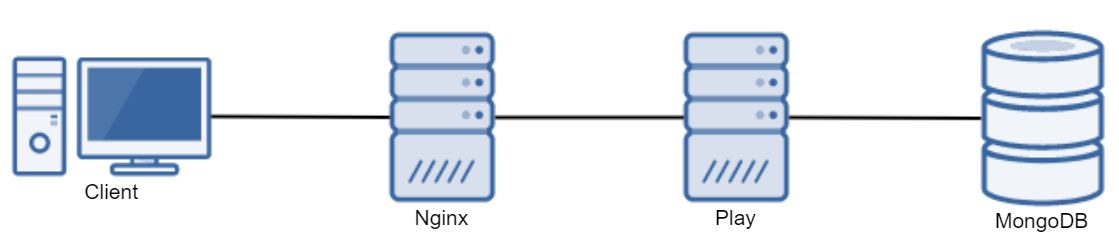
\includegraphics[width=1.0\textwidth]{images/Architecture.png}
		\caption{Overview of the architecture of Uber for Bikes}
		\label{arch}
	\end{figure}

For our webserver we have written the main component in Scala. Scala is a functional programming language supporting high scalability. We used the Play framework which fits our purposes very well as it is designed for developing web applications.  As well as this. it ensures the integration with the database and the other components.

For our project we used the MongoDB database with a Scala ReactiveMongo driver. ReactiveMongo provides fully non-blocking and asynchronous I/O operations. ReactiveMongo is designed to avoid any kind of blocking request. Every operation returns immediately, freeing the running thread and resuming execution when it is over.

In the frond-end, Angular and Bootstrap are used for providing a nice user interface. The UI serves a simple purpose: Renting and unrenting bikes. The main view of the UI is a Google Maps view. It is currently set to the location of Groningen, but could eventually be used to show the region where the user resides.
In our project we use an external third party service. The service of Google is needed to convert a textural representation of a location into the corresponding geographical representation of the GPS system. This conversion is done via the Google Maps API.


\subsection{Docker swarm}

Docker swarm is a tool that enables high scalability and fault-tolerance. With Docker swarm, it is possible to run applications on a cluster of virtual or physical machines. If one of the nodes or one of the containers fails the other keep functioning and can handle the requests that are send to them. For every service, there are two modes available, global and replicated. If  the replicated mode is used, the user can define the number of replicas of each container. If the global mode is used, every node in the cluster runs one instance of the service. In our application, we use global mode for all the services, which means that if we run our application on two (virtual) machines, each machine will have one instance of every service running on it.
